\clearpage\section{Chapter 11: Writing Large Programs}

This chapter describes language features, techniques, and software tools
that play a supporting role in developing large programs and libraries
of reusable code. You can write large programs or libraries without
these tools; the tools just make certain tasks easier. These facilities
are not specific to object-oriented programs. However, they serve the
same target audience since one of the primary benefits of
object-orientation is to reduce the difficulty of developing large
programs.

In the case of Unicon, {\textquotedbl}large{\textquotedbl} might mean
any program so complex that it is not self-explanatory without any
special effort. This includes all programs over a few thousand lines in
size, as well as shorter programs with complex application domains, and
those written by multiple authors or maintained by persons other than
the original author.

Writing and maintaining large programs poses additional challenges not
encountered when writing small programs. The need for design and
documentation is greater, and the challenge of maintaining the
correspondence between design documents and code is more difficult.
Design patterns can help you with the design process, since they
introduce easily recognizable idioms within a design. The more familiar
the design is, the less cognitive load is imposed by the task of
understanding it.

This chapter shows you how to:

\begin{itemize}
\item Understand the difference between abstract and concrete classes
\item Use design patterns to simplify and improve software designs
\item Organize programs and libraries into packages
\item Generate HTML indices and reference documentation for your code
\end{itemize}

\subsection{Abstract Classes}

In programming languages, it turns out there are at least two very
different kinds of things referred to by the word
{\textquotedbl}class{\textquotedbl}. Most classes denote a data type,
of which there are one or more instances. The word class is also used
to denote a general category of objects, of which there are no actual
instances. Such classes are called \index{abstract class}abstract
classes. \index{class!abstract}Abstract classes are used by defining
subclasses which do have instances. In a small program you might not
run into a need for abstract classes, but if you write a large
object-oriented program, or your small program uses someone
else{\textquotesingle}s large object-oriented class library, you are
likely to need to understand abstract classes.

The whole idea of class and inheritance originated by analogy from
biology, but if you think about it, biology uses a host of different
terms to denote categories (phylum, family, genus, etc.), that are
distinct from the term that denotes a class of instances (species).
There are plenty of instances of species \textit{Homo sapiens}, but
there are no instances of a genus \textit{Homo}, there are only
instances of \textit{Homo}{\textquotesingle}s subclasses. Similarly, if
you are designing software to model the behavior of cars and trucks,
you may identify a lot of shared behavior and place code for it in a
superclass Vehicle, but there are no instances of Vehicle, only its
subclasses.

In a larger inheritance graph (or tree) most classes may well be
abstract. It may be those classes (primarily leaves) of which there are
actual instances that are special and deserve a different term besides
{\textquotedbl}class{\textquotedbl}. We could easily think of all
classes as abstract by default, and refer to classes that have
instances as {\textquotedbl}concrete classes{\textquotedbl} or
\ {\textquotedbl}instantiation classes{\textquotedbl}. The analogy to
biology would be better served by such terminology. But for better or
for worse, most software engineers will have to live with
{\textquotedbl}abstract class{\textquotedbl} and
{\textquotedbl}class{\textquotedbl} to denote general categories and
instantiable categories, respectively.

Numerous larger and more concrete examples of abstract classes appear in
the Unicon GUI class library, described in Chapter 17. Some classes,
such as Button, denote general categories of widgets that have code and
behavior in common (such as the fact that you can click them). There
are no instances of Button, there are only subclasses such as
\textsf{TextButton}, \textsf{IconButton}, and \textsf{CheckBox}, that
may be instantiated. In larger applications, the code sharing (or
duplication avoidance) of abstract classes may be compelling, but like
all uses of inheritance they do require you to read and understand
multiple bodies of code (the class and all its superclasses) in order
to use the class effectively.

\subsection{Design Patterns}

Class and function libraries provide good mechanisms for \index{code
reuse}code reuse, and \index{inheritance}inheritance helps with code
reuse in some situations. But in large programs it is desirable to
reuse not just code, but also successful designs that capture the
relationships between classes. Such design reuse is obtained by
identifying \index{design patterns}\textit{design patterns} with known
successful uses in a broad range of application domains. For example,
the practice of using pipes to compose complex filters from more
primitive operations has been successfully used in compilers, operating
system shells, image processing, and many other application areas.
Every programmer should be familiar with this pattern.

The field of software design \index{patterns, design}patterns still
quite young. Practitioners are producing simple catalogs of patterns,
such as the book \textit{Design Patterns}, by Erich Gamma, Richard
Helm, Ralph Johnson, and John Vlissides. When the field is more mature
it will include syntactic and/or semantic rules for how patterns are
combined to form higher-order patterns, as is the case for building
architecture. This section presents a few classic patterns and their
implementation in Unicon.

At best, this discussion of patterns may whet your appetite to go read
more about the subject. In addition to their design reuse value,
patterns also provide software developers with a common vocabulary for
discussing recurring design concepts. The judicious use of one or more
abstract classes seems to be a recurring theme throughout most of the
design patterns identified by Gamma et al.

\subsubsection{Singleton}

Perhaps the simplest design pattern is the \index{singleton}singleton,
describing a class of which exactly one \index{instance!class}instance
is required. Singletons are interesting because they are related to
\textit{packages}, a language feature described later in this chapter.
A \index{package}package is a mechanism for segregating a group of
global objects so that their names do not conflict with the rest of the
program. This segregation is similar to that provided by object
encapsulation; a package is similar to a class with only one instance.

Consider as an example a global table that holds all the records about
different employees at a small company. There are many instances of
class \textsf{Employee}, but only one instance of class
\textsf{EmployeeTable}. What is a good name for this instance of
\textsf{EmployeeTable}, and how can you prevent a second or subsequent
instance from being created? The purpose of the singleton pattern is to
answer these questions. 

In Unicon, one interesting implementation of a singleton is to replace
the \index{constructor!class}constructor procedure (a global variable)
by the instance. Assigning an object instance to the variable that used
to hold the constructor procedure allows you to refer to the instance
by the name of the singleton class. It also renders the constructor
procedure inaccessible from that point on in the
program{\textquotesingle}s execution, ensuring only one instance will
be created.

\iconcode{
class EmployeeTable(...) \\
initially \\
\>   EmployeeTable := self \\
end
}

\noindent
There are undoubtedly other ways to implement singleton classes.

\subsubsection{Proxy}

A \index{proxy pattern}proxy is a {\textquotedbl}stand-in{\textquotedbl}
for an object. The proxy keeps a \index{reference}reference to the
object it is replacing, and implements the same interface as that
object by calling the object{\textquotesingle}s version of the
corresponding method each time one of its methods is invoked. Figure
11-1 shows a proxy serving a client object in lieu of the real object.

\bigskip

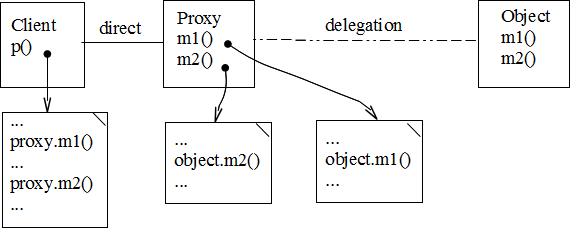
\includegraphics[width=5.8in,height=2.9in]{ub-img/proxy.png}

{\sffamily\bfseries Figure 11-1:}
{\sffamily The Proxy Pattern}

\bigskip

Proxies are used when the original object cannot or should not be
invoked directly. If the object is on a remote machine, the proxy can
take care of network communication and hide the location of the object
from the clients. As another example, the original object may be
instantiated lazily - it may be a large object that is not loaded into
memory unless one of its operations is invoked.

Similar to both of the preceding examples, mobile objects might be
implemented using proxies. If several machines are running a
computation jointly and communicating, some gigantic object might be
kept on one machine at a time. In applications with strong locality of
reference, whenever a machine needs to do a call on the gigantic object
it might do hundreds of calls on that object. In that case the object
should move from wherever it is, to the machine where it is needed. The
rest of the program does not need to be aware of whether the object is
local, remote, or mobile; it just interacts with the proxy instance.

\iconcode{
class gigantic(x1,x2,...,x1000) \\
\>   method invoke() \\
\>   \ \ \ ... \\
\>   end \\
initially \\
\>   \# Gigantic object{\textquotesingle}s state is loaded from network \\
end \\
class proxy(g) \\
\>   method invoke() \\
\>   \ \ \ /g := gigantic() \\
\>   \ \ \ return g.invoke() \\
\>   end \\
\>   method depart() \\
\>   \ \ \ g := \&null \\
\>   end \\
end
}

\subsubsection{Chain of Responsibility}

This pattern is similar to a proxy, in that an object is
\textit{delegating} one or more of its methods to a second object. It
is not presented in detail, but its similarity to proxies is mentioned
because many design patterns in the Gamma book seem incredibly similar
to each other; reading the book is like having d�j� vu all over again.
Perhaps there ought to be some kind of orthogonality law when it comes
to patterns.

The difference between a chain of responsibility and a proxy is that the
proxy forwards \textit{all} method invocations to the
{\textquotedbl}real{\textquotedbl} object, while in a chain of
responsibility, the object may handle some methods locally, and only
delegate certain methods to the next object in the chain. Also, proxies
are normally thought of as a single level of indirection, while the
chain of responsibility typically involves multiple linked objects that
jointly provide a set of methods. The following example illustrates a
chain of responsibility between a data structure object (a cache) and
an \textsf{Image} class that knows how to perform a computationally
intensive resolution enhancement algorithm.

\iconcode{
class Image(...) \\
\>   method enhance\_resolution(area) \\
\>   \ \ \ \# enormous computation... \\
\ \\
\>   end \\
initially \\
\>   \# ... lots of computation to initialize lots of fields \\
end \\
\ \\
class hirez\_cache(s, t) \\
\>   method enhance\_resolution(area) \\
\>   \ \ \ if member(t,area) then \{ \# proxy handles \\
\>   \ \ \ \ \ \ return t[area] \\
\>   \ \ \ \ \ \ \} \\
\>   \ \ \ \# else create the gigantic instance \\
\>   \ \ \ /im := image() \\
\>   \ \ \ return t[area] := im.enhance\_resolution(area) \\
\>   end \\
initially \\
\>   t := table() \\
\>   \# Insert some known values for otherwise enormous computation. \\
\>   \# Don{\textquotesingle}t need im if user only needs these values. \\
\>   t[1] := 1 \\
\>   t[2] := 1 \\
end
}

The instance of class Image is not created until one is needed, and
image{\textquotesingle}s method \textsf{enhance\_resolution()} is not
invoked for previously discovered results. Of course,
\textsf{enhance\_resolution()} must be a pure mathematical function
that does not have any side effects for this caching of results to be
valid.

\subsubsection{Visitor}

The \index{visitor pattern}visitor pattern is a classic exercise in
generic algorithms. It is fairly common to have a structure to
\index{traverse}traverse, and an operation to be performed on each
element of the structure. Writing the code for such a traversal is the
subject of many data structure texts. In fact, if you have one
operation that involves traversing a structure, there is a good chance
that you have (or will someday need) more than one operation to perform
for which the same traversal is used. Figure 11-2 illustrates the
visitor pattern.

\bigskip

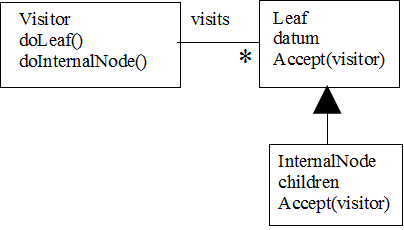
\includegraphics[width=4.0in,height=2.25in]{ub-img/visitor.png}

{\sffamily\bfseries Figure 11-2:}
{\sffamily The Visitor Pattern}

\bigskip

The visitor pattern says you can separate out the traversal algorithm
from the operation performed at each element of the structure, and
reuse the traversal on other operations. The following code illustrates
this separation of traversal (implemented by method \textsf{Accept()})
from visitation (implemented by methods \textsf{DoLeaf()} and
\textsf{DoInternalNode()} in the visitor). Where there is one kind of
visitor there may be many, and in that case, class Visitor may be an
abstract class, instantiated by many concrete Visitor
\index{subclass}subclasses that have the same method names but do not
share code. Note also that this code example allows for heterogeneous
structures: the Visitor just defines a
{\textquotedbl}Do...{\textquotedbl} method for each type of node in the
structure.

\iconcode{
class Visitor() \\
\>   method DoLeaf(theLeaf) \\
\>   \ \ \ \# ... visit/use theLeaf.datum \\
\>   end \\
\>   method DoInternalNode(theNode) \\
\>   \ \ \ \# ... visit/use theNode.datum \\
\>   end \\
end \\
class Leaf(datum) \\
\>   method Accept(v) \\
\>   \ \ \ v.DoLeaf(self) \\
\>   end \\
end \\
class InternalNode : Leaf(children) \\
\>   method Accept(v) \\
\>   \ \ \ every (!children).Accept(v) \\
\>   \ \ \ v.DoInternalNode(self) \\
\>   end \\
end
}

Executing a traversal from a root object looks like
\textsf{root.Accept(myvisitor)} where \textsf{myvisitor} is an instance
of some \textsf{Visitor} class. The point of the Visitor pattern is
that you can define different Visitor classes. For example, here are
Visitors to print a tree, and to calculate and store the heights of all
nodes in the \index{tree}tree:

\iconcode{
class Printer() \\
\>   method DoLeaf(theLeaf) \\
\>   \ \ \ writes(theLeaf.datum, {\textquotedbl} {\textquotedbl}) \\
\>   end \\
\>   method DoInternalNode(theNode) \\
\>   \ \ \ writes(theNode.datum, {\textquotedbl} {\textquotedbl}) \\
\>   end \\
end \\
class Heights() \\
\>   method DoLeaf(theLeaf) \\
\>   \ \ \ theLeaf.datum := 1 \\
\>   end \\
\>   method DoInternalNode(theNode) \\
\>   \ \ \ theNode.datum := 0 \\
\>   \ \ \ every theNode.datum {\textless}:= (!children).datum \\
\>   \ \ \ theNode.datum +:= 1 \\
\>   end \\
end
}

\subsection{Packages}

In large programs, the global name space becomes crowded. You can create
a disaster if one of your undeclared local variables uses the same name
as a built-in function, but at least you can memorize the names of all
the built-in functions and avoid them. Memorization is no longer an
option after you add in hundreds of global names from unfamiliar code
libraries. You may accidentally overwrite some other
programmer{\textquotesingle}s global \index{global}variable, without
any clue that it happened.

Packages allow you to partition and protect the global \index{name
space}name space. A package is similar to a
{\textquotedblleft}singleton{\textquotedblright} class with only one
instance. Every global declaration (variables, procedures, records, and
classes) is {\textquotedbl}invisible{\textquotedbl} outside the
\index{package}package, unless imported explicitly.

\subsubsection[The package declaration]{The \textrm{\textmd{package}}
declaration}
A package declaration specifies that all global symbols within a source
file belongs to a package. \ The package declaration looks similar to
the \index{link}link declaration. You provide the package name an
identifier or a string filename:

\iconcode{
package foo}

or

\iconcode{
package {\textquotedbl}/usr/local/lib/icon/foo{\textquotedbl}}

There can be only one package declaration in a source file. It need not
be at the beginning of the source file, but this is conventional.
Within a package, global names defined inside the package are
referenced normally. Global names outside the package are not visible
by default. Here is an example source file that declares some globals
and adds them to a package.

\bigskip

\iconcode{
\# pack1.icn \\
package first \\
procedure my\_proc() \\
\>   write({\textquotedblleft}In my\_proc{\textquotedblright}) \\
end \\
class SomeClass() \\
\>   method f() \\
\>   \ \ \ write({\textquotedblleft}In
SomeClass.f{\textquotedblright}) \\
\>   end \\
end
}

When this code is compiled, the information that package first contains
the symbols \textsf{my\_proc} and \textsf{SomeClass} is recorded into a
database and that using package \textsf{first} implies linking in
\textsf{pack1.u} along with any other files that are part of package
\textsf{first}. In order to prevent name conflicts the compiler also
applies a name mangling process to the global symbols, described below.

\subsubsection[The import declaration]{The \textmd{import} declaration}
To access symbols within another package, use the import declaration,
which has the following syntax:

\iconcode{
import foo}

This causes the compiler to look up the package in its database and
identify its symbols. Import declarations use the IPATH
\index{environment variable!IPATH}environment variable in the same way
as do link declarations. In particular, an import declaration
\textit{is} a link declaration, augmented with \index{scope}scope
information about the names defined in the package.

\subsubsection[Explicit Package References]{Explicit Package References}
Sometimes, two imported packages may define the same symbol, or an
imported symbol conflicts with a global declaration in one of your
files. To resolve these problems, you can explicitly specify the
package to use for particular symbol references. For example, if
packages first and second both define a procedure named write, then

\iconcode{
import first, second \\
procedure main() \\
\>   first::write()\ \ \ \ \# calls write() in package first \\
\>   second::write()\ \ \ \ \# calls write() in package second \\
\>   ::write()\ \ \ \ \ \ \# calls the global write() \\
end
}

The use of the \textsf{::} operator on its own is a useful way to refer
to a global procedure from within a class that has a method of the same
name, as in

\iconcode{
class Abc(x) \\
\>   method write() \\
\>   \ \ \ ::write({\textquotedblleft}Abc x={\textquotedblright}, x) \\
\>   end \\
end
}

In this example, omitting the \textsf{::} would cause the
\textsf{write()} method to call itself until the program runs out of
memory and produces a runtime error.

\subsubsection{Name Conflicts and Name Mangling}

The purpose of packages is to reduce name conflicts, especially
accidental ones. You will get a link error if you declare the same name
twice in the same package. You will get a \index{compile}compile error
if you try to import a package that contains a variable that is already
declared. In Unicon, unlike Arizona Icon, you will also get a warning
message if you declare a global variable of the same name as a built-in
function, or assign a new value to such a name. Often this is done on
purpose, and it shows off the flexibility of the language. But other
times when it happens by accident, it is a disaster. Such warnings can
be turned off with the \textsf{{}-n} option to the \textsf{unicon}
compiler.

Under the hood, packages are implemented by simple name mangling that
prefixes the package name and a pair of underscores onto the front of
the declared name. You can easily defeat the package mechanism if you
try, but the reason to mention the name mangling is so you can avoid
variable names that look like names from other packages.

A similar \index{name mangling}name mangling constraint applies to
classes. Also, the compiler reserves field names \textsf{\_\_s} and
\textsf{\_\_m} for internal use; they are not legal class field names.
Identifiers consisting of \textsf{\_}\textsf{\textit{n}}, where
\textit{n} is an integer are reserved for Unicon temporary variable
names. Finally, for each class \textsf{foo} declared in the
user{\textquotesingle}s code, the names \textsf{foo},
\textsf{foo\_\_state}, \textsf{foo\_\_methods}, and
\textsf{foo\_\_oprec} are reserved, as are the names \textsf{foo\_bar}
corresponding to each method \textsf{bar} in class \textsf{foo}. 

\subsubsection{Compilation Order and the Unidep Tool}

When possible, you should compile all files in a package before you
import that package. Even if you do, if multiple source files belong to
the same package, the order in which they are compiled is significant.
Consider the following code in three source files:

\iconcode{
\# order1.icn \\
package demo \\
procedure first() \\
\>   write({\textquotedblleft}first{\textquotedblright}) \\
end \\
\ \\
\# order2.icn \\
package demo \\
procedure second() \\
\>   write({\textquotedblleft}second{\textquotedblright}) \\
\>   first() \\
end \\
\ \\
\# order3.icn \\
import demo \\
procedure main() \\
\>   second() \\
end
}

Files \textsf{order1.icn} and \textsf{order2.icn} belong to a package
demo, which is used by \textsf{order3.icn}. You can rightly guess that
order3.icn should be compiled after \textsf{order1.icn} and
\textsf{order2.icn}, but does it matter which of them is compiled
first? If \textsf{order2.icn} is compiled first,
Unicon{\textquotesingle}s database does not know symbol first is part
of the package, and does not mangle the name; if you compile these
files out of order you will get a runtime error.

The brute force solutions you have available to you are: to always place
all of a package in the same source file, or to compile the files
twice. Neither of these options is especially appealing. The symbol
references in each package{\textquotesingle}s files form a graph of
dependencies on the other files in the same package. As long as this
graph is acyclic, a correct order can be calculated. Unidep is a
program that automates this task and generates a \ makefile specifying
the dependencies in build rules. For example, given the program above,
and the following makefile:

\iconcode{
order: order1.u order2.u order3.u \\
\ \ unicon -o order order1.u order2.u order3.u \\
\%.u: \%.icn \\
\ \ unicon -c \$*
}

Running the command {\textquotedblleft}unidep order1.icn order2.icn
order3.icn{\textquotedblright} will append the required additional
dependencies. In this case these are:

\iconcode{
order1.u: order1.icn \\
order2.u: order2.icn order1.u \\
order3.u: order3.icn order2.u \\
}

With these dependencies added, the makefile will compile the files in
the correct order. You will want to add a rule to invoke Unidep from
the makefile, and rerun it when your program changes significantly.

\subsection{HTML documentation}

\index{iplweb}Iplweb is an Icon documentation generator, inspired
loosely by \index{Java}Java{\textquotesingle}s \index{JavaDoc}JavaDoc
program, and based on an \index{HTML}HTML{}-generating program called
iplref, by Justin Kolb. Iplweb depends on your program being in
{\textquotedbl}IPL normal form{\textquotedbl}, which is to say that
\index{comment}comments in your source files should be in the format
used in the Icon Program Library. From these comments and the
signatures of procedures, methods, records, and classes, Iplweb
generates \index{reference!documentation}reference documentation in
HTML format.

This approach produces reference documentation automatically, without
altering the original source files. Run Iplweb early, and run it often.
It is common for reference documentation to diverge over time from the
\index{source code}source code without such a tool. \ It is especially
suitable for documenting the interfaces of procedure and class
libraries. What it doesn{\textquotesingle}t help with is the
documentation of how something is implemented. It is designed primarily
for the users, and not the maintainers, of library code.

\section*{Summary}

Writing and maintaining large programs poses additional challenges not
encountered when writing small programs. The need for design and
documentation is greater, and the challenge of maintaining the
correspondence between design documents and code is more difficult.
Design patterns can help you with the design process, since they
introduce easily recognizable idioms or sentences within a design. The
more familiar the design is, the less cognitive load is imposed by the
task of understanding it.

Packages have little or nothing to do with design patterns, but they are
just as valuable in reducing the cognitive load required to work with a
large program. Packages are not just a source code construct. They
actually do play a prominent role in software design notations such as
UML. From a programmer{\textquotesingle}s point of view, packages
protect a set of names so that their associated code is more reusable,
without fear of conflicts from other reusable code libraries or the
application code itself.
